\section{Alkali Vapor Dispensing and Non-Evaporable Gas Gettering}
\label{sec:neg_dispenser}
Prior to the final hermetic sealing of the laser-written vapor cell, a
small solid-state non-evaporable getter (NEG) dispenser pill 
is precisely positioned within the
micromachined reservoir cavity, as shown in Figure~\ref{fig:lwvc_neg}. The cell enclosure is
subsequently sealed inside a controlled chamber filled with atmospheric
pressure nitrogen (\ce{N2}) buffer gas, ensuring an ultra-low oxygen (\ce{O2})
concentration below \SI{6}{ppm} to avoid trapping reactive oxygen species within
the internal cavities \cite{lucivero2022}. Throughout this initial assembly
stage, the solid-state pill remains completely stable and chemically inert,
preventing any premature release of reactive species before the hermetic
enclosure is fully secured.
\begin{figure}[h]
    \centering
    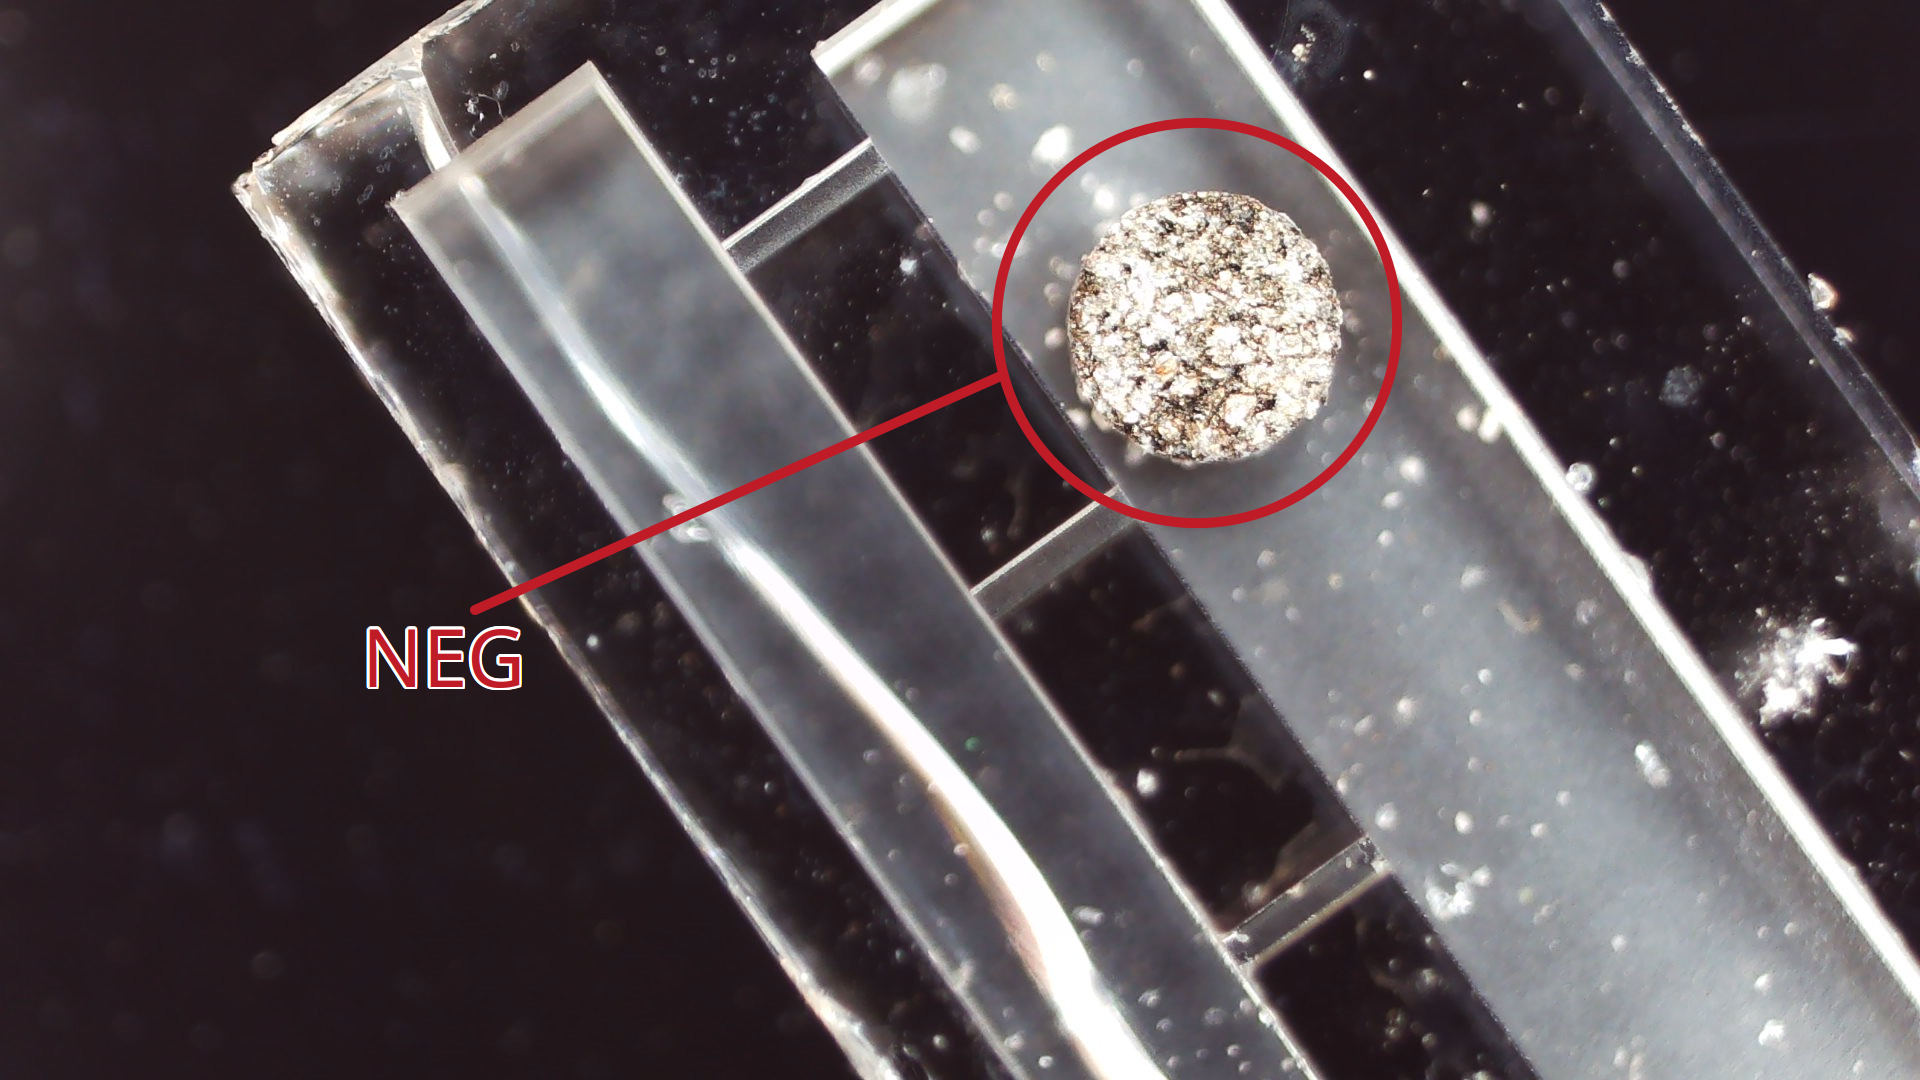
\includegraphics[width=\linewidth]{Images/NEG_in_lwvc.png}
    \caption{Optical micrograph of a LWVC following the physical 
    integration of the NEG dispenser within the reservoir, captured prior to the optical 
    contact bonding stage. The visible defects on the sample are a consequence of extensive 
    prototyping and handling tests, and do not reflect the nominal fabrication quality.}
    \label{fig:lwvc_neg}
\end{figure}
The dispenser pill consists of a compressed powder mixture combining an
alkali-metal chromate, such as rubidium chromate (\ce{Rb2CrO4}) or cesium
chromate (\ce{Cs2CrO4}), with a specialized reducing agent composed of
\SI{84}{\percent} zirconium (Zr) and \SI{16}{\percent} aluminum (Al) by weight
\cite{scherer2012}. While these dispenser materials are traditionally activated
in macroscopic vacuum systems via ohmic heating to drive the pellet into a temperature range
of \SI{400}{\celsius} to \SI{800}{\celsius} \cite{scherer2012}.
Under this thermal activation, the chemical reduction
of the rubidium chromate by the zirconium matrix follows the stoichiometry:
\begin{equation}
    \mathrm{4Rb_2CrO_4 + 5Zr \rightarrow 8Rb\uparrow + 2Cr_2O_3 + 5ZrO_2}
    \label{eq:reduction_rb}
\end{equation}
Simultaneously, the interaction between the activated zirconium matrix and the
nitrogen (\ce{N2}) buffer gas dictates the final internal pressure environment.
This active surface
permanently chemisorbs excess internal \ce{N2} buffer gas via the formation of
stable zirconium nitride (\ce{ZrN}) solid solutions \cite{knapkiewicz2018}. 

The LWVC architecture utilizes a non-invasive laser activation
mechanism to trigger the reduction-oxidation process post-sealing \cite{lucivero2022}.
To initiate the vapor release, a high-power and tightly focused laser beam
is targeted directly onto the opaque surface of the
small pill for a few seconds. This localized
optical absorption rapidly drives the internal pellet temperature into the
required activation window  \cite{lucivero2022}. During this process,
the NEG undergoes a
chemical reduction that releases elemental alkali vapor, while simultaneously
acting as a getter material that sorbs other
chemically active gases created during the reaction, preventing them from
contaminating the internal chamber atmosphere \cite{scherer2012}.
Following the reaction, the liberated rubidium or cesium vapor
diffuses into the sensing chambers of the vapor cell, while the buffer gas 
is partially absorbed. 


